
\documentclass{PoS}
\usepackage{amsmath}

\title{Single top quark production measurements at the LHC: t-channel}

\ShortTitle{Single top quark production measurements at the LHC: t-channel}

\author{
    \speaker{Matthias Komm}, on behalf of the ATLAS and CMS collaborations\\
    Universite Catholique de Louvain (UCL) (BE)\\
    E-mail: \email{Matthias.Komm@cern.ch}
}

\abstract{
At the LHC, single top quarks are predominately produced via the $t$-channel. Measuring the properties of the production process provides a crucial probe of the theory of electroweak interactions. This paper reviews recent results on cross section measurements and coupling structure studies in pp collisions by the ATLAS and CMS collaborations at center-of-mass energies of 7, 8, and 13~TeV.
}

\FullConference{
    8th International Workshop on Top Quark Physics\\
    14-18 September, 2015\\
    Ischia, Italy
}

\begin{document}

\section{Introduction}
The production and decay of single top quarks via $t$-channel involves electroweak interactions at leading order (LO). The high mass of the top quark allows it to decay to on-shell W bosons before hadronization becomes relevant. This allows to measure a variety of standard model~(SM) properties such as the CKM matrix element $\mathrm{V_{tb}}$ and the parity-violating V-A coupling structure.

In the following, the latest results by the ATLAS and CMS collaborations are reviewed.

\section{Cross section measurements at 8~TeV}
Precise measurements of the $t$-channel single top quark cross section at 8~TeV have been accomplished at the LHC in pp collisions by the ATLAS and CMS collaborations~\cite{atlas-xsec8,cms-xsec8} utilizing data that corresponds to approximately $20~\mathrm{fb}^{-1}$. For the measurements, events with an isolated muon or electron and two jets are selected where one jet is required to pass the threshold of dedicated b-tagging algorithms. The cross section is measured using a binned maximum-likelihood~(ML) fit to a discriminating variable. CMS exploits the pseudorapidity distribution of the non b-tagged jet that is produced in the forward detector region for single top quark events~(Fig.~\ref{fig:fit-xsec-8}a) whereas ATLAS combines multiple observables into one powerful discriminant by training a neural network~(Fig.~\ref{fig:fit-xsec-8}b).

\begin{figure}[htbp]
\begin{center}
\parbox{0.52\textwidth}{\centering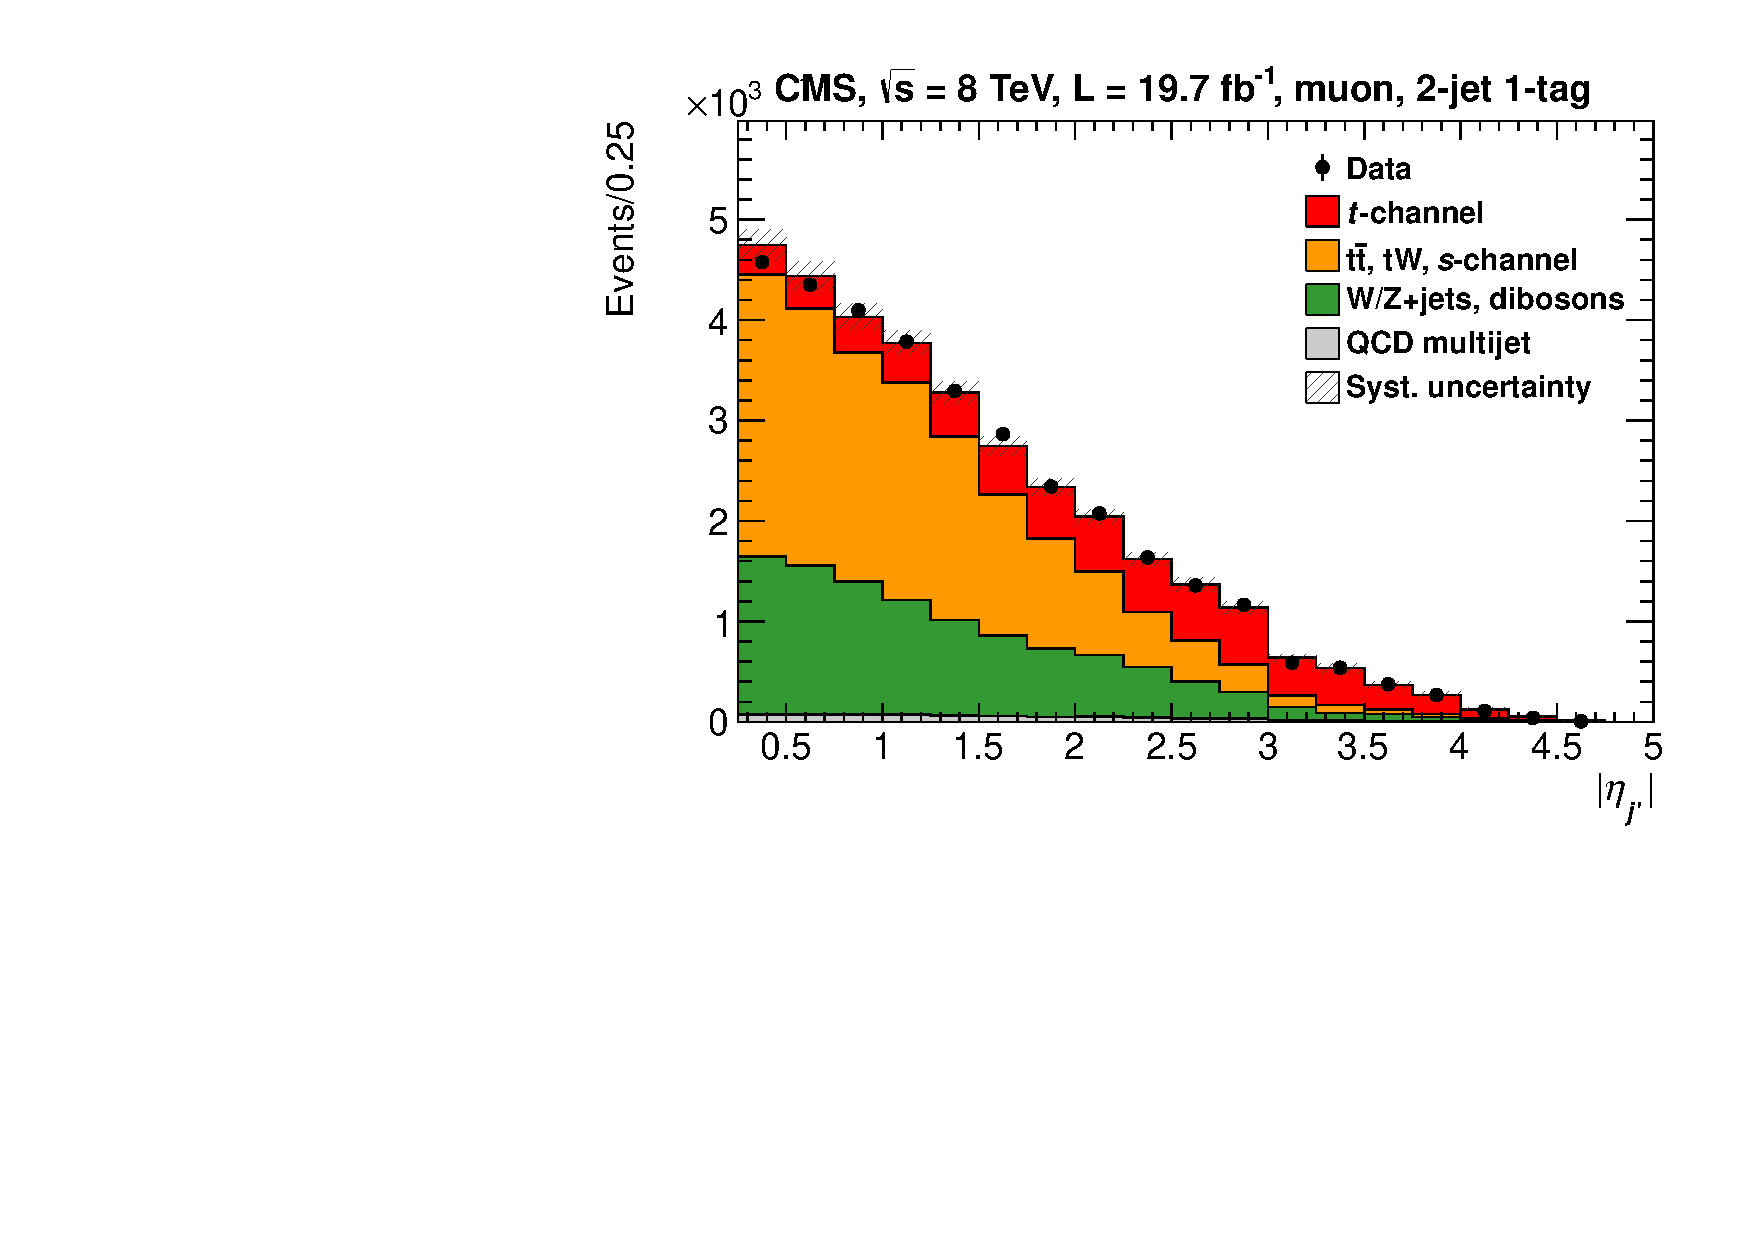
\includegraphics[width=0.51\textwidth]{cms_xsec8/etamuon.pdf}}
\parbox{0.47\textwidth}{\centering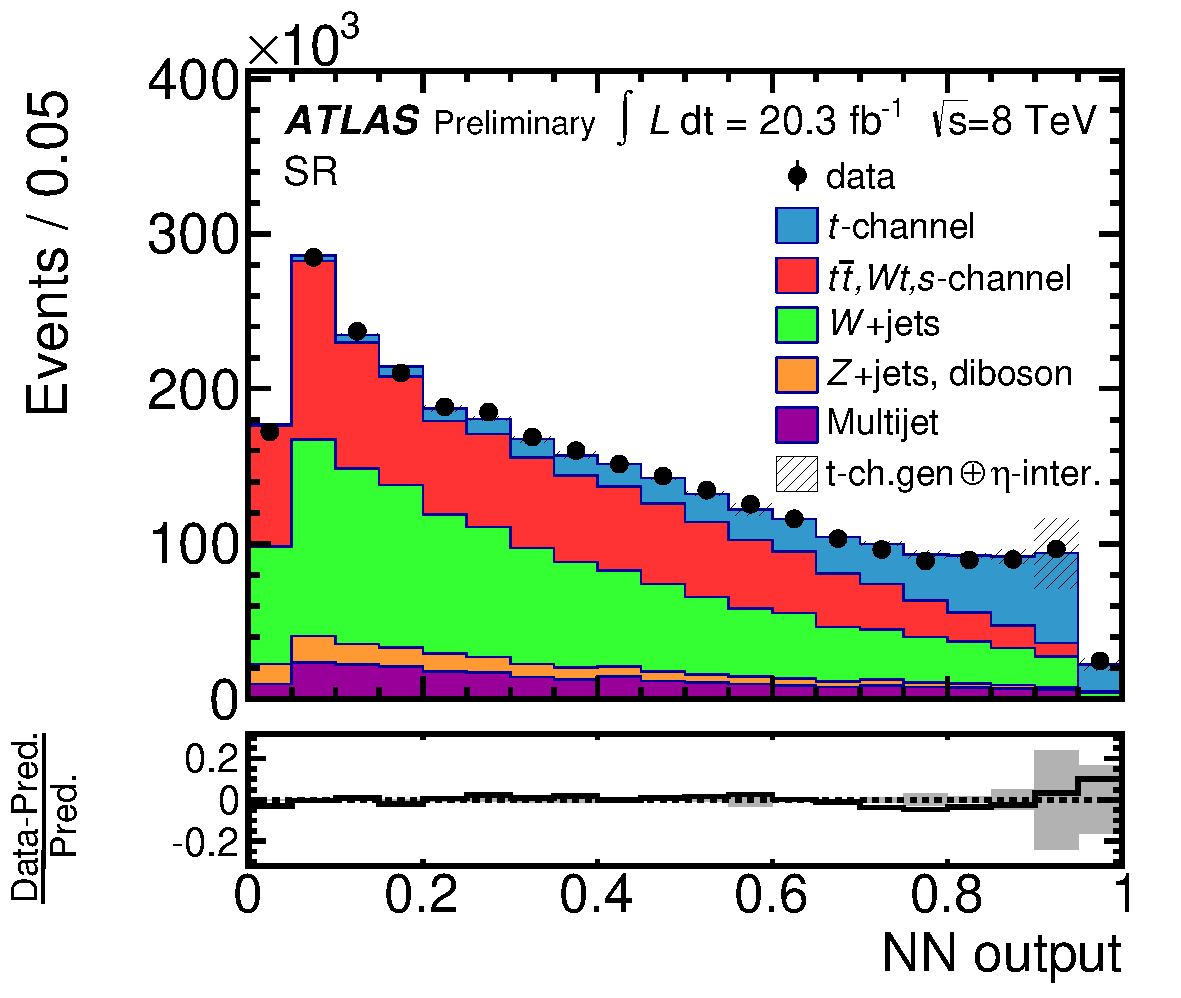
\includegraphics[width=0.46\textwidth]{atlas_xsec8/nnoutput.pdf}}\\
\parbox{0.52\textwidth}{\centering (a)}
\parbox{0.47\textwidth}{\centering (b)}
\end{center}
\caption{\label{fig:fit-xsec-8}Distributions of discriminating observables used to measure the single top quark cross section: (a)~pseudorapidity of the non b-tagged jet used by CMS~\cite{cms-xsec8} and (b)~neural network discriminant used by ATLAS~\cite{atlas-xsec8}.}

\end{figure}

The measured inclusive cross section is used to set a limit on the CKM matrix element $|\mathrm{V_{tb}}|\simeq\sqrt{\sigma_\mathrm{obs.}/\sigma_\mathrm{theo.}}$. This procedure makes no assumptions on the number of quark generations or the unitariy of the CKM matrix. The measured cross sections at 8~TeV together with the extracted limits on $\mathrm{|V_{tb}|}$ are 
\begin{align}
\sigma_{t\mbox{-}\mathrm{ch.}}^\mathrm{ATLAS}&=82.6\pm1.2\mathrm{(stat)}\pm12.0\mathrm{(syst)}~\mathrm{pb}, &\Rightarrow |\mathrm{V_{tb}}|>0.78~\mathrm{(95\%~CL,~8~TeV)}, \\
\sigma_{t\mbox{-}\mathrm{ch.}}^\mathrm{CMS}&=83.6\pm2.3\mathrm{(stat)}\pm7.4\mathrm{(syst)}~\mathrm{pb} &\Rightarrow |\mathrm{V_{tb}}|>0.92~\mathrm{(95\%~CL,~7+8~TeV)}
\end{align}

which are compatible with the expectation of $83.9_{-0.2}^{+0.6}\mathrm{(scale)}~\mathrm{pb}$ at next-to-next-to-leading order (NNLO)~\cite{Brucherseifer-xsec8}.

In addition to the inclusive cross section, the fiducial cross section has been measured as well~\cite{atlas-xsec8,CMS-PAS-TOP-15-007}. It provides a deep test of the theory by restricting the measurement only to the detector acceptance. The advantage is that fiducial measurements are not affected by theoretical uncertainties that account for extrapolations into an experimentally unprobed phase space.





\section{Charge ratio measurements}
The cross section ratio $\sigma(t)/\sigma(\bar{t})$ has also been measured~\cite{cms-xsec8,atlas-charge7}. It is particular sensitive to the parton distribution functions~(PDF). Figure~\ref{fig:charge-ratio} shows measurements by CMS~(8~TeV) and ATLAS~(7~TeV) compared to different PDF sets. Similar tensions in both measurements for some sets are observed. 

\begin{figure}[htbp]
\begin{center}
\parbox{0.47\textwidth}{\centering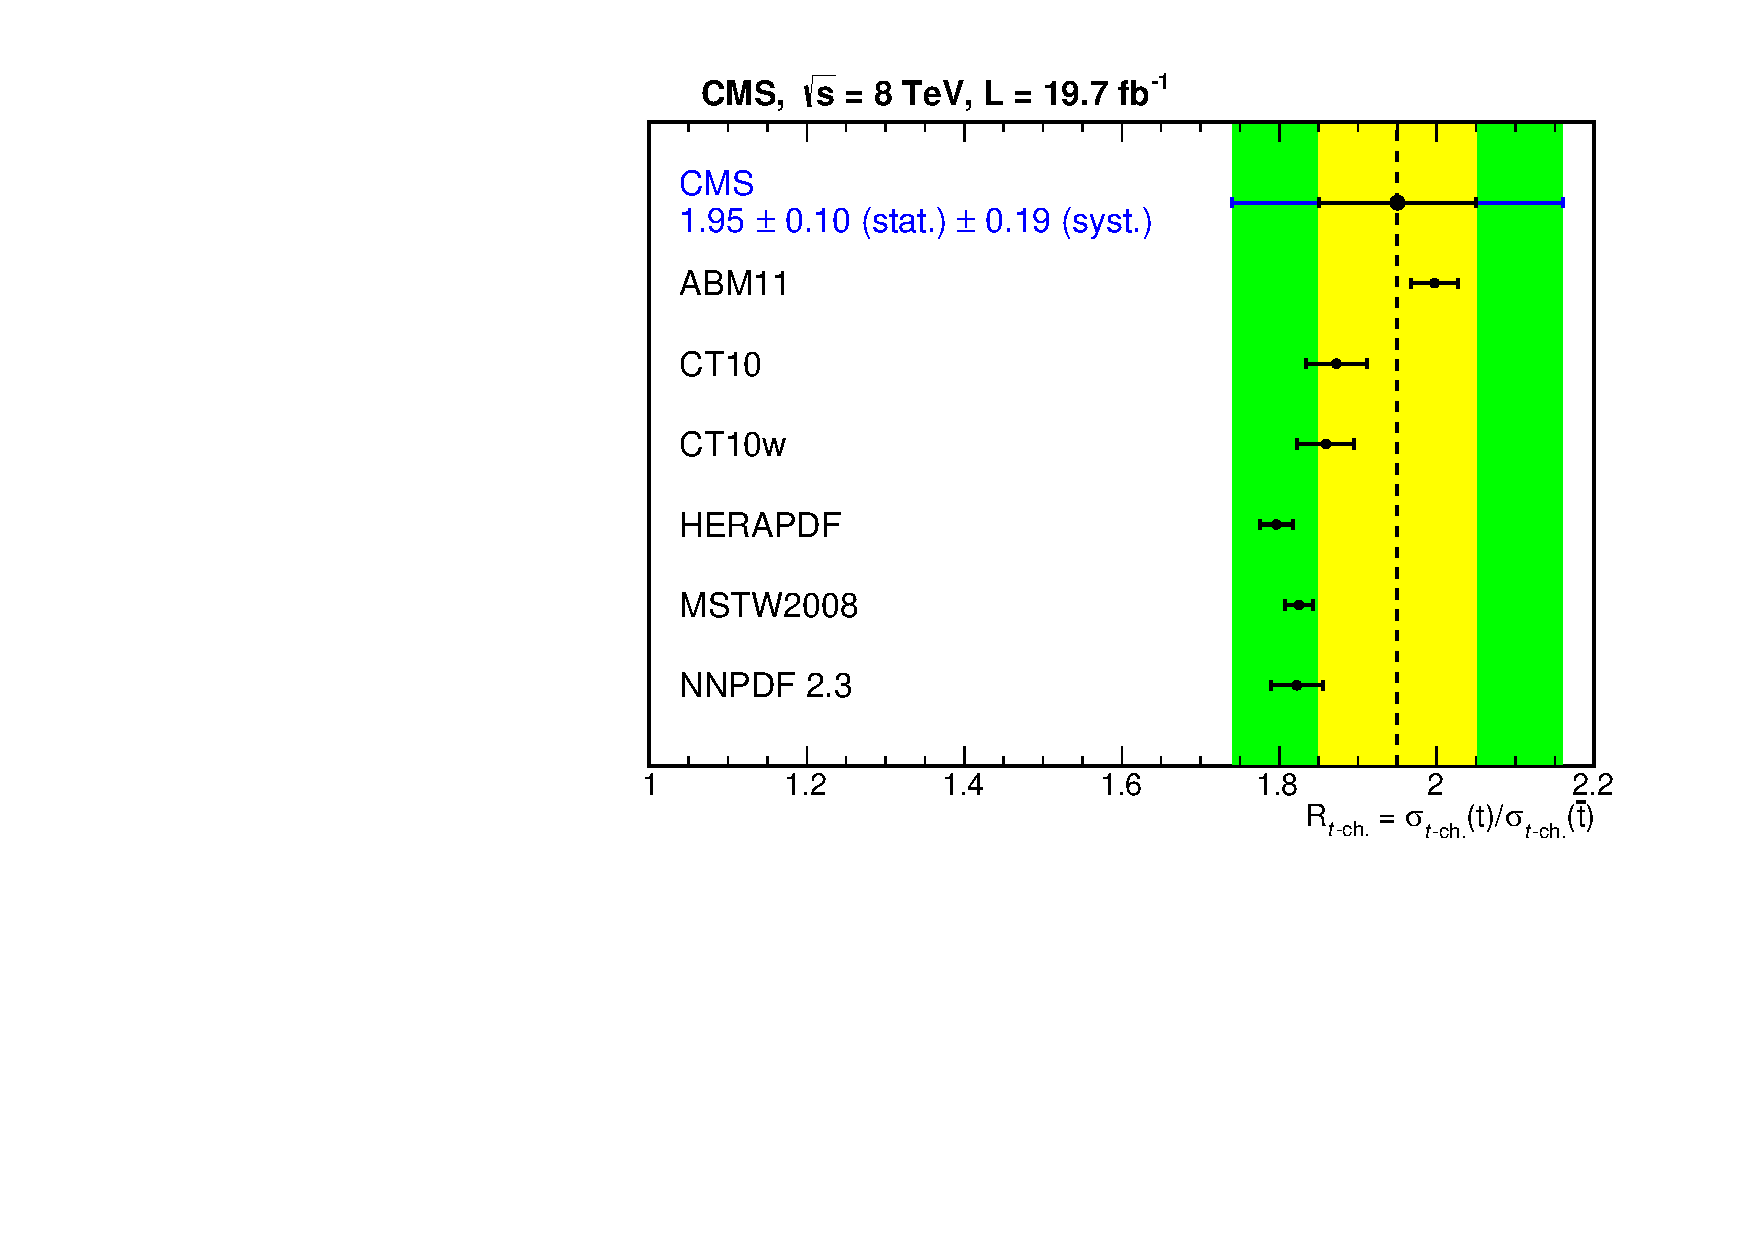
\includegraphics[width=0.46\textwidth]{cms_xsec8/charge.pdf}}
\parbox{0.47\textwidth}{\centering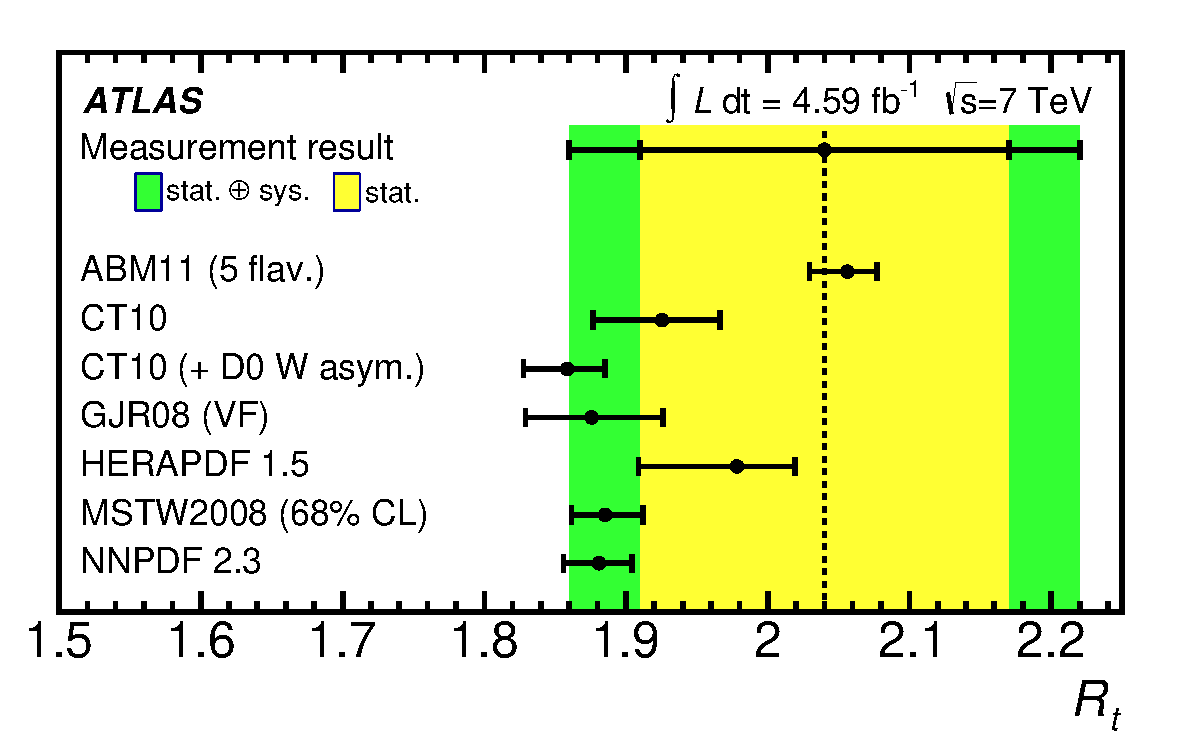
\includegraphics[width=0.46\textwidth]{atlas_charge7/charge.pdf}}\\
\parbox{0.47\textwidth}{\centering (a)}
\parbox{0.47\textwidth}{\centering (b)}
\end{center}
\caption{\label{fig:charge-ratio}Cross section ratio for top quark over antiquark production: (a)~result by CMS at 8~TeV~\cite{cms-xsec8} and (b)~result by ATLAS at 7~TeV~\cite{atlas-charge7}.}

\end{figure}

\section{Electroweak coupling structure}
Single top quark events allow to probe the electroweak V-A structure because of the Wtb vertex in production and decay. Deviations can be characterized in terms of anomalous Wtb couplings that arise from effective dimension-six operators. A novel analysis technique to set limits on anomalous couplings has been developed by ATLAS~\cite{atlas-anomcoupl}. It utilizes a double differential distribution with respect to the polar~(Fig.~\ref{fig:angles}a) and azimuthal~(Fig.~\ref{fig:angles}b) angles of the lepton in the reconstructed W boson rest frame.

\begin{figure}[htbp]
\begin{center}
\parbox[t]{0.45\textwidth}{\centering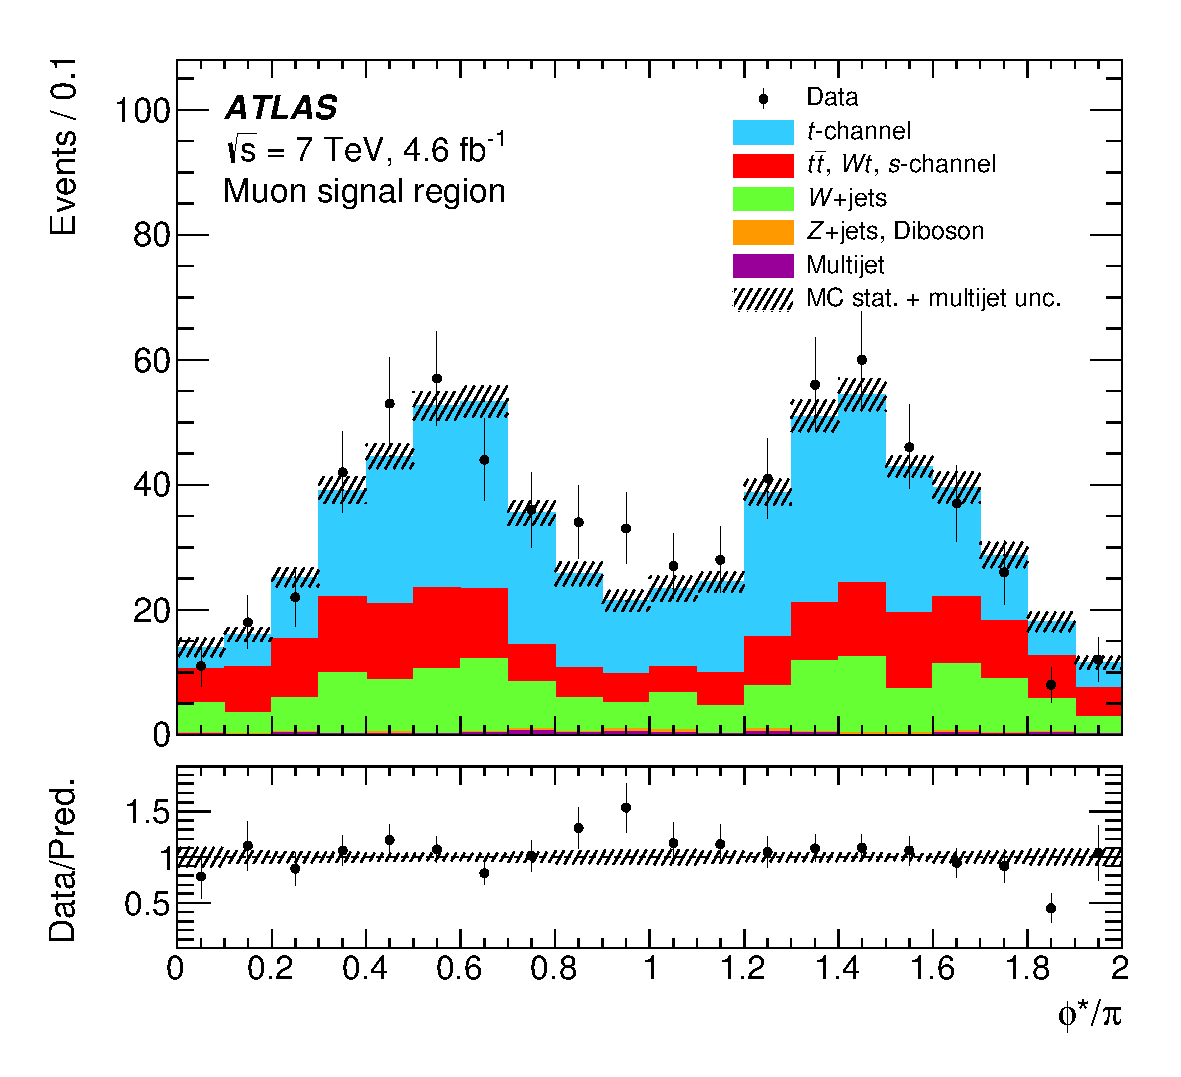
\includegraphics[width=0.43\textwidth]{atlas_anomcoupl/phi.pdf}}
\parbox[t]{0.45\textwidth}{\centering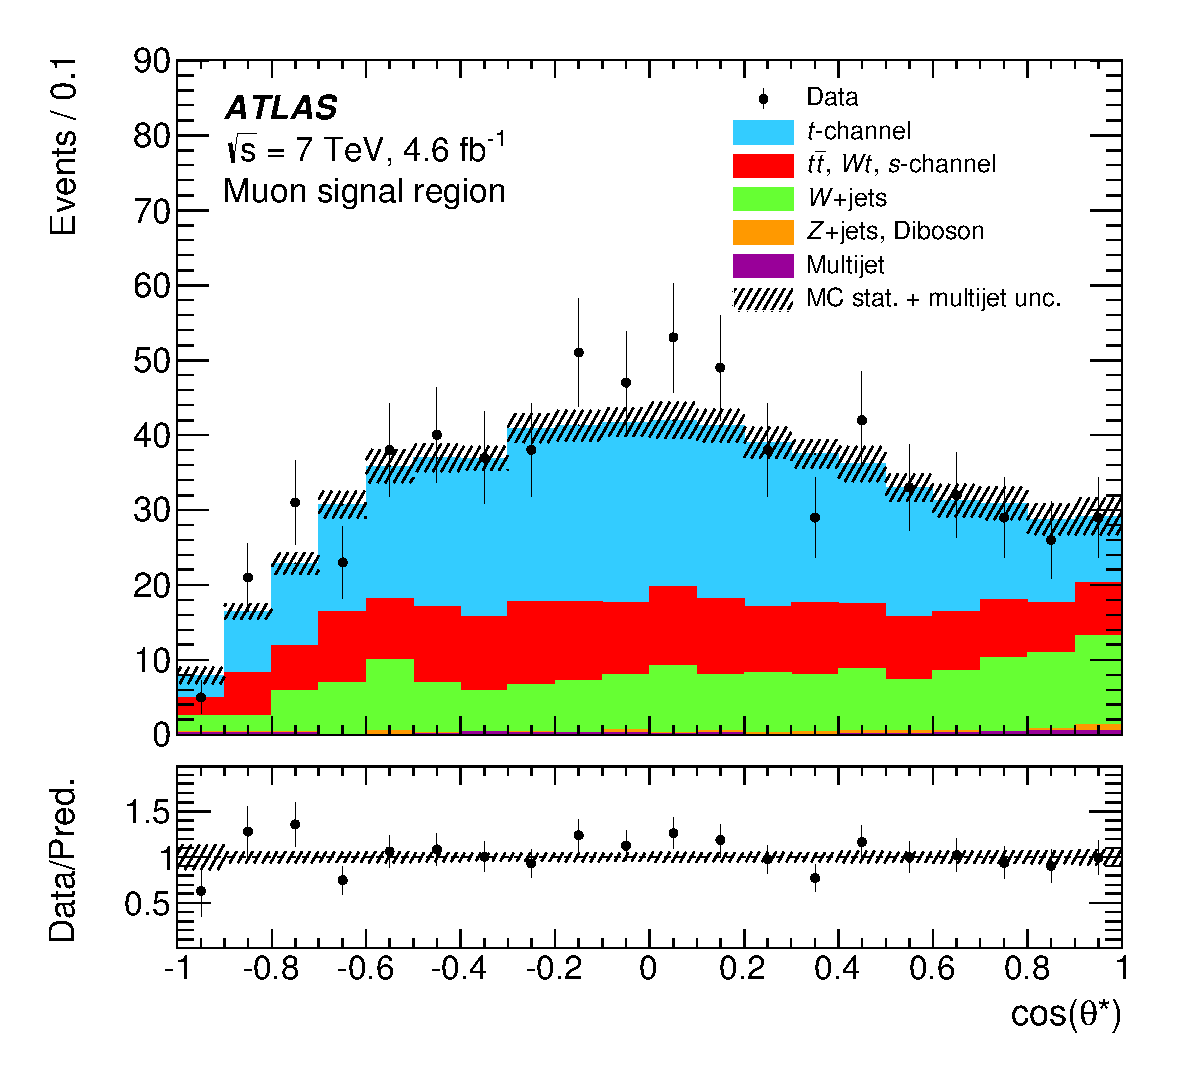
\includegraphics[width=0.43\textwidth]{atlas_anomcoupl/theta.pdf}}\\
\parbox[t]{0.45\textwidth}{\centering (a)}
\parbox[t]{0.45\textwidth}{\centering (b)}\\\medskip
\parbox[t]{0.99\textwidth}{\centering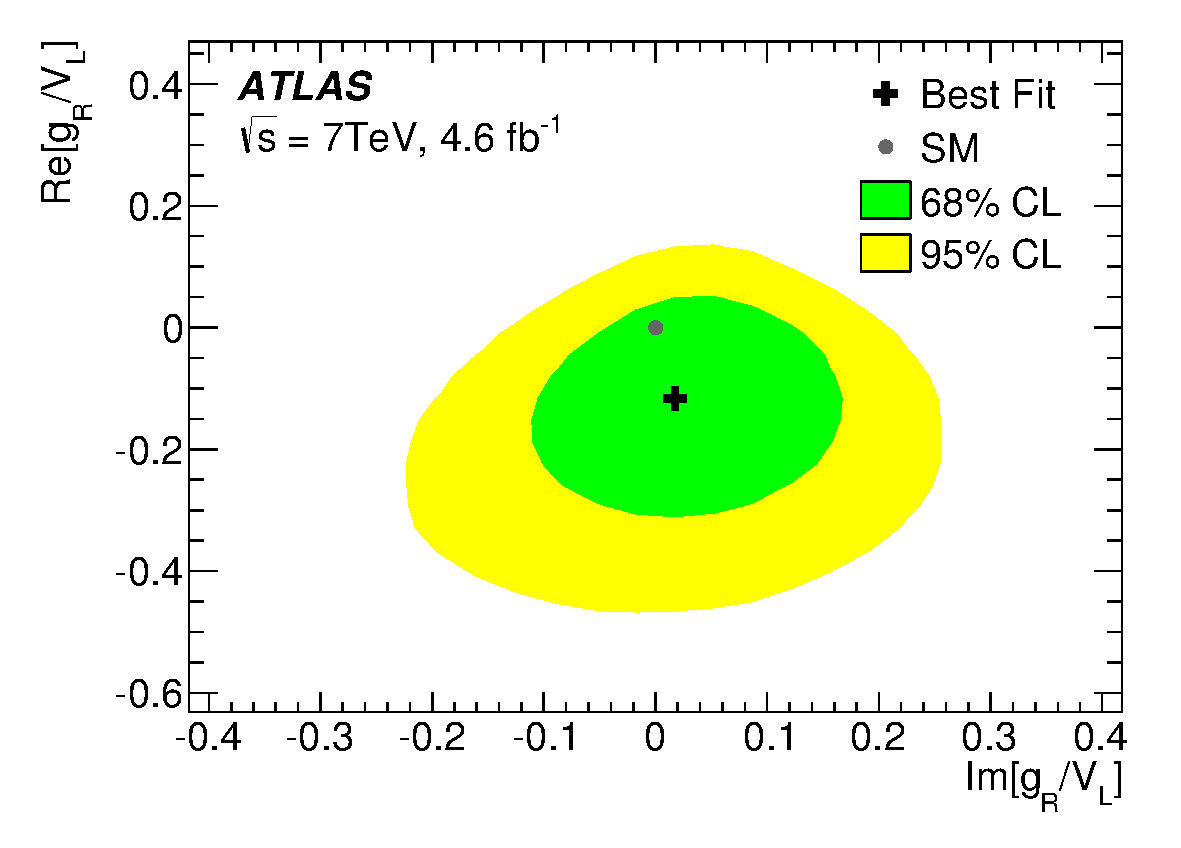
\includegraphics[width=0.43\textwidth]{atlas_anomcoupl/limits.pdf}\\(c)}
\end{center}
\caption{\label{fig:angles}Distributions of (a)~the polar angle and (b)~the azimuthal angle of the lepton in the W boson rest frame, and (c)~the inferred limits on the anomalous tensor-like right-handed Wtb coupling over the SM coupling. Figures are taken from Ref.~\cite{atlas-anomcoupl}.}
\end{figure}

An event-based likelihood is constructed for both angles using an analytical folding model that accounts for finite resolution, acceptance and reconstruction inefficiencies. Limits on the real and imaginary part of the right-handed tensor anomalous coupling~\cite{minimal-anom-set} with respect to the left-handed vector-like SM coupling, $g_{R}/V_{L}$, are inferred and shown in Fig.~\ref{fig:angles}c. In particular, the analysis sets a new limit on the imaginary part of $\mathrm{Im}(g_{R}/V_{L})\in[-0.17,0.23]$ at 95\% CL. The imaginary part of this quantity was never measured before.


\section{Early cross section measurement at 13~TeV}

After the long shutdown, the LHC has been restarted at a new center-of-mass energy of 13~TeV. An early single top quark $t$-channel cross section measurement has been performed by CMS~\cite{CMS-PAS-TOP-15-004} with the first recorded data that corresponds to $42~\mathrm{pb}^{-1}$.
The analysis strategy follows closely the previous measurement at 8~TeV. Events with one isolated muon and two jets are selected where one jet is required to be b-tagged. The QCD multijet background is estimated by modeling its shape from data with inverted muon isolation and fitted to the transverse W boson mass distribution as shown in Fig.~\ref{fig:singletop13}a. The pseudorapidity distribution of the forward, non b-tagged jet~(Fig.~\ref{fig:singletop13}b) is used to measure the single top quark cross section using a binned ML fit.
\begin{figure}[htbp]
\begin{center}
\parbox[t]{0.34\textwidth}{\centering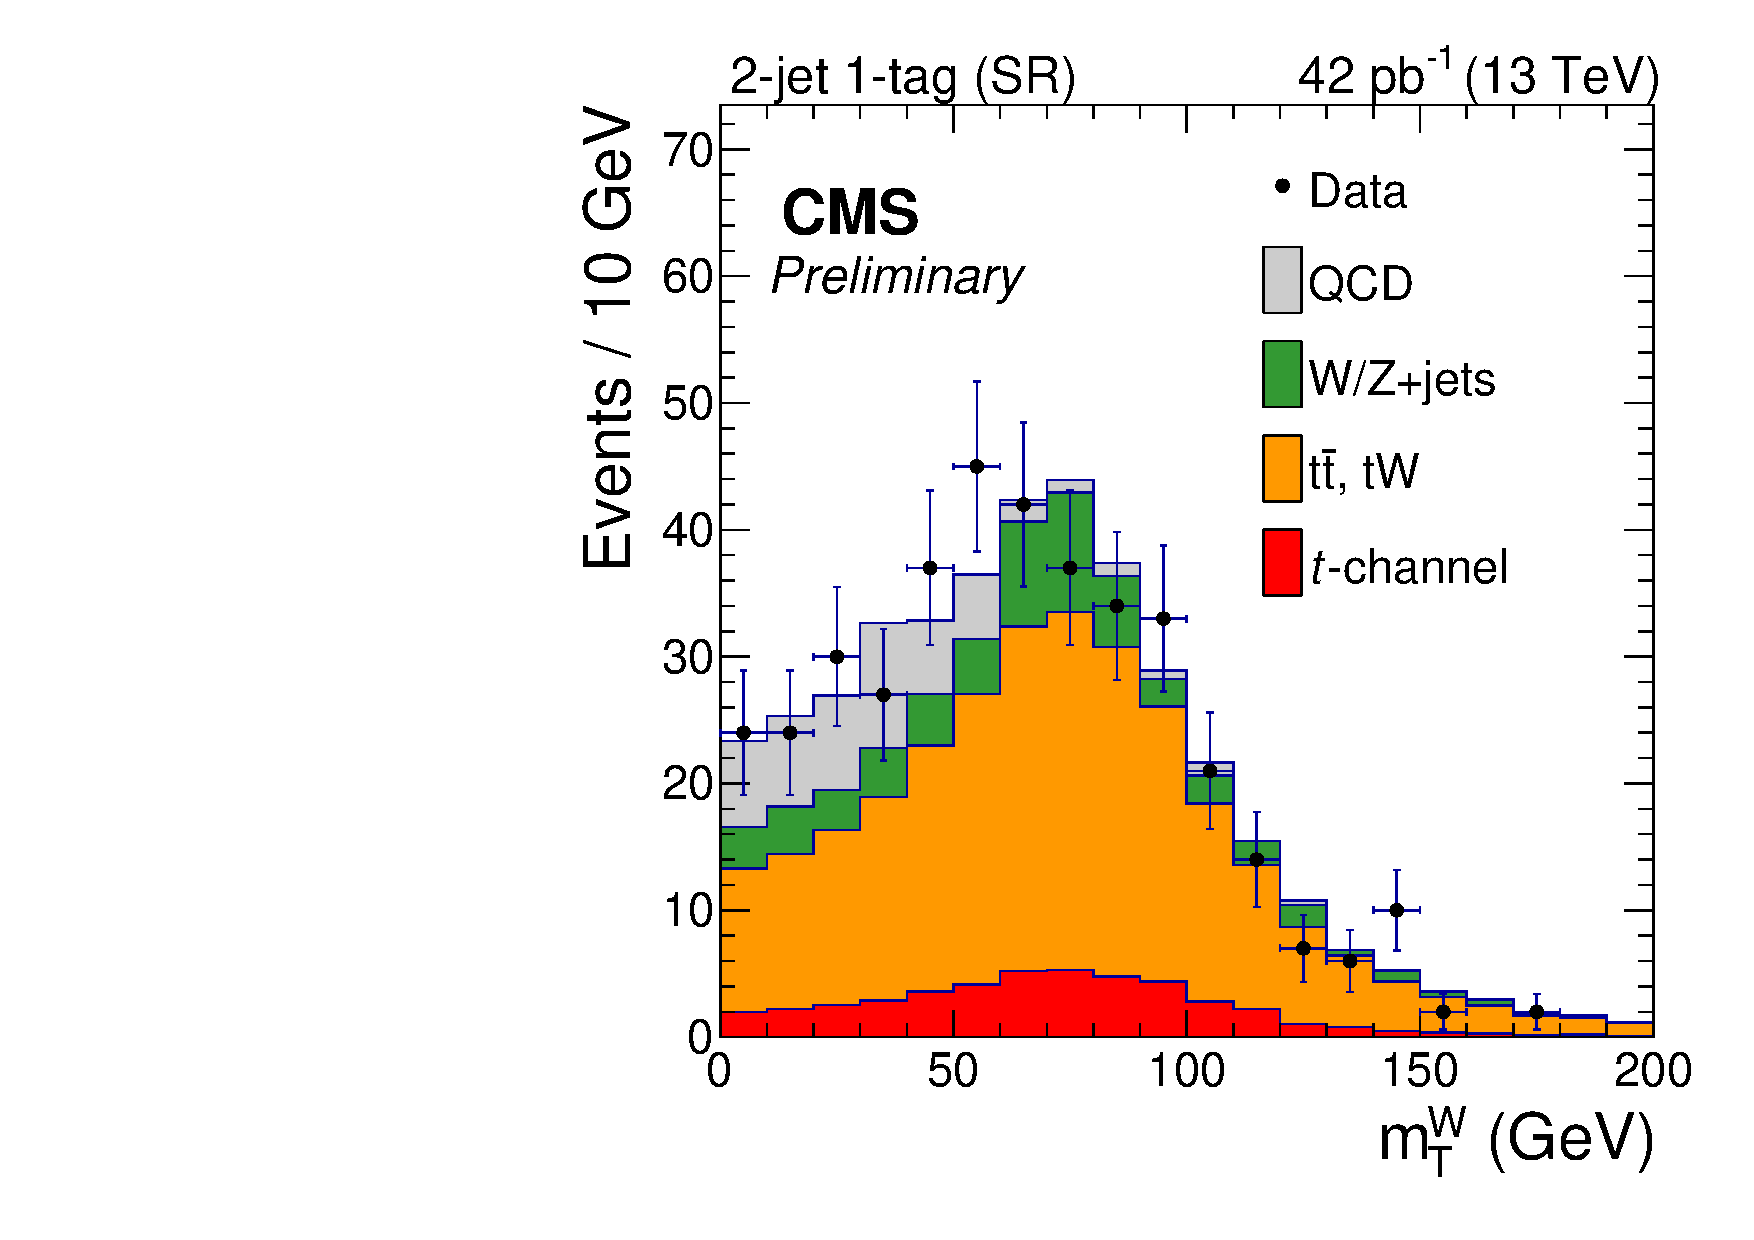
\includegraphics[width=0.33\textwidth]{cms_xsec13/mtw.pdf}}
\parbox[t]{0.34\textwidth}{\centering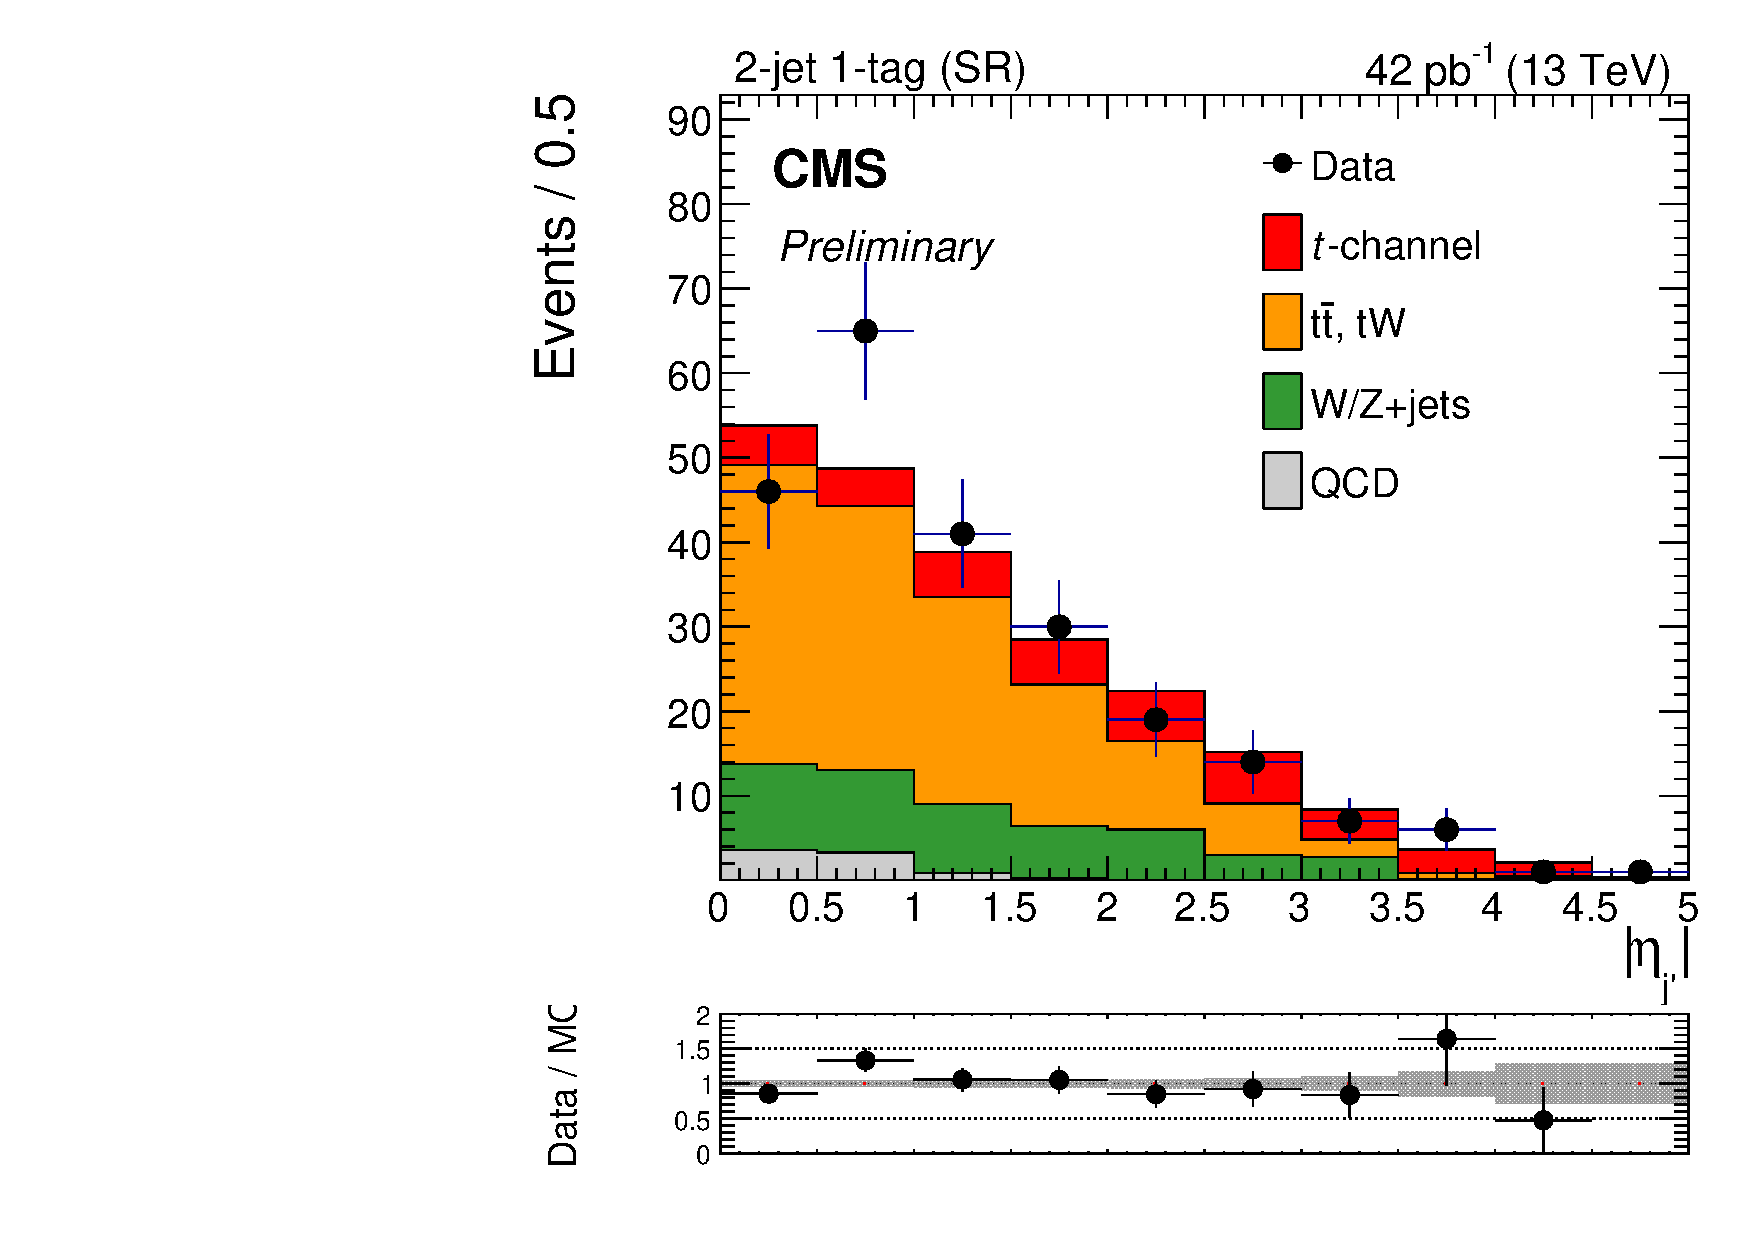
\includegraphics[width=0.33\textwidth]{cms_xsec13/mu2j1t.pdf}}\\
\parbox[t]{0.34\textwidth}{\centering (a)}
\parbox[t]{0.34\textwidth}{\centering (b)}\\\medskip
\parbox[t]{0.99\textwidth}{\centering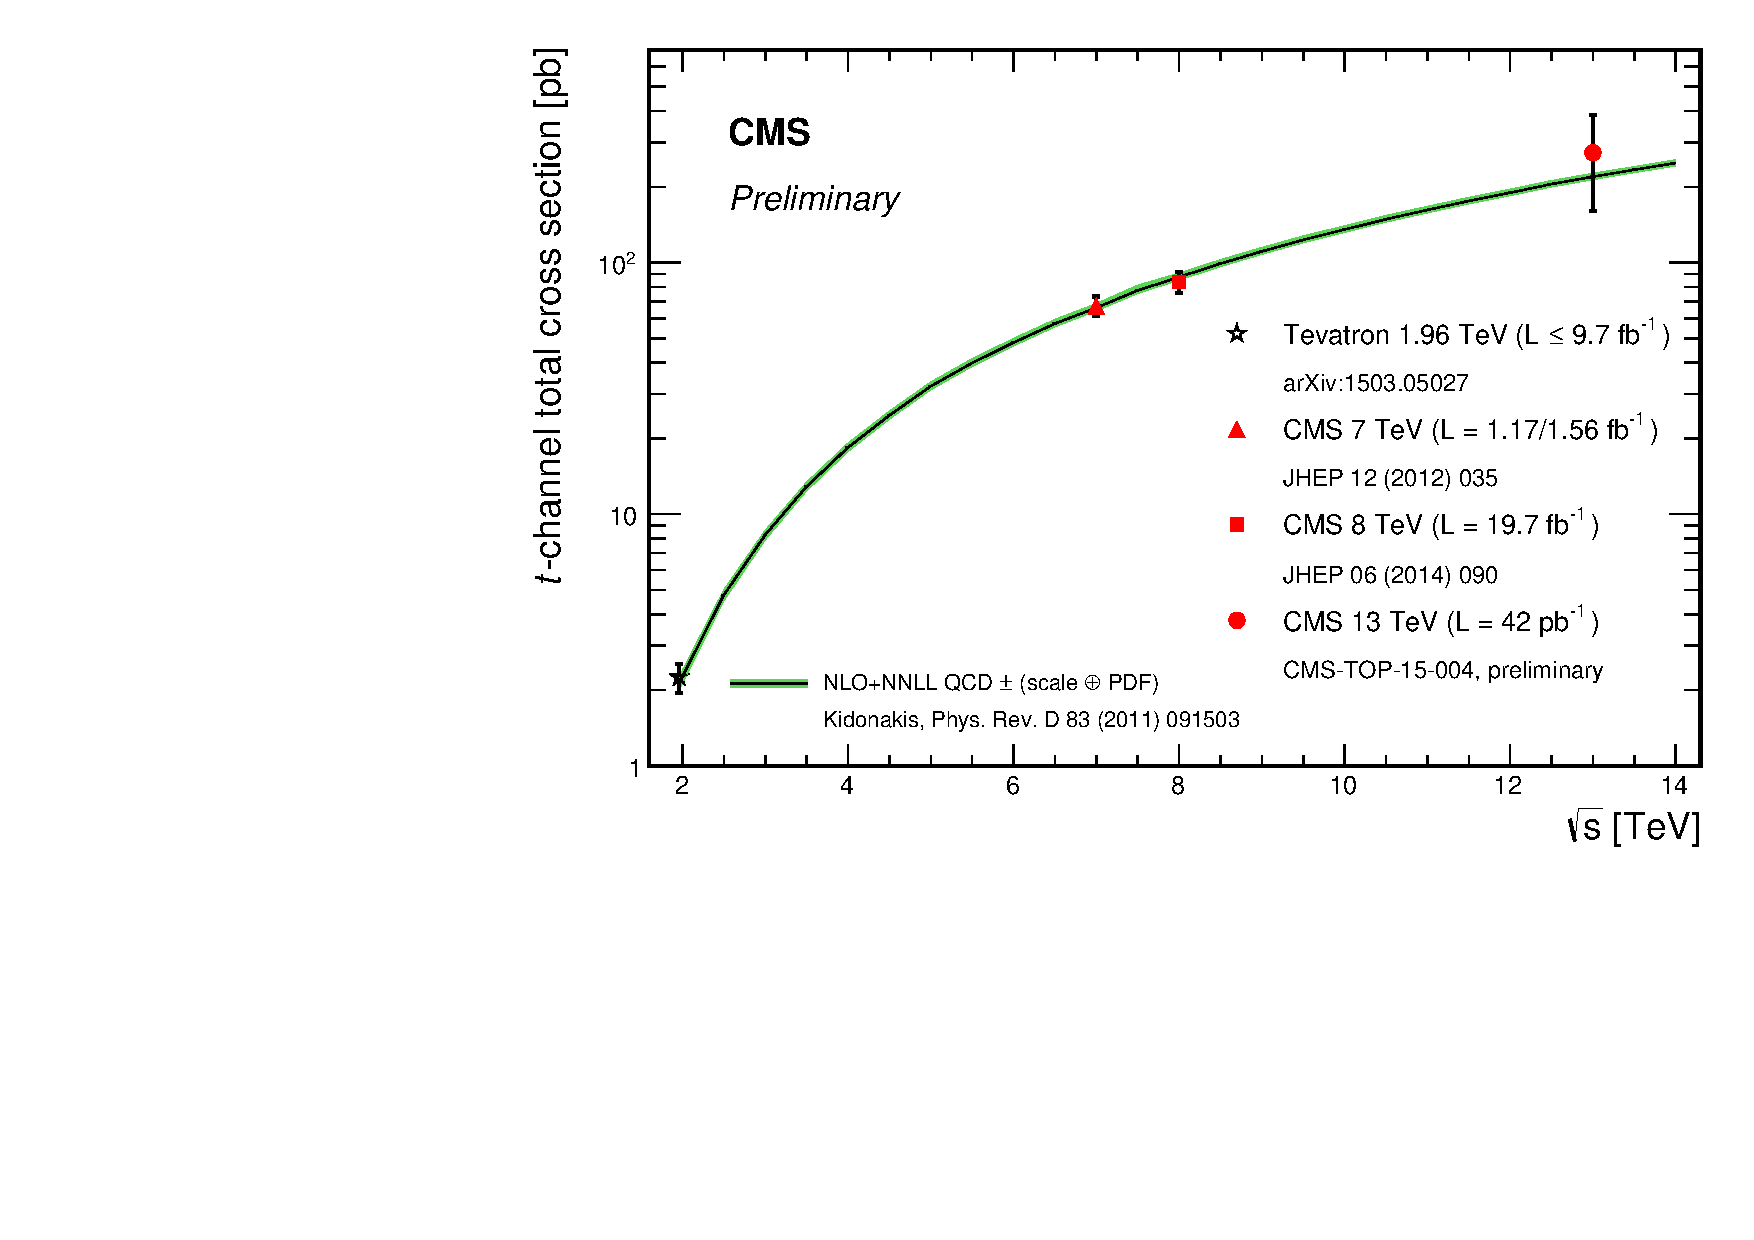
\includegraphics[width=0.42\textwidth]{cms_xsec13/xsec.pdf}\\(c)}
\end{center}
\caption{\label{fig:singletop13}Distributions of (a)~the transverse W boson mass, (b)~the pseudo rapidity of the forward, non b-tagged jet, and (c)~a comparison with theory of the cross section measurements by CMS. Figures are taken from Ref.~\cite{CMS-PAS-TOP-15-004}.}
\end{figure}

The major sources of uncertainty are the data statistics~(36\%), jet energy calibration~(17\%) and luminosity~(12\%).
The early single top quark $t$-channel analysis at 13~TeV yields a cross section of
\begin{equation}
\sigma_{t\mbox{-}\mathrm{ch.}}=274~\mathrm{pb}\pm98\mathrm{(stat)}\pm52\mathrm{(syst)}\pm33\mathrm{(lumi)}~\mathrm{pb}.
\end{equation}

The result agrees within uncertainties with the expectation of $218_{-2}^{+5}\mathrm{(scale)}\pm5\mathrm{(PDF)}~\mathrm{pb}$ at approximate NNLO~\cite{Kidonakis-8tev}. A comparison with theory is shown in Fig.~\ref{fig:singletop13}c together with measurements at 7~and 8~TeV by CMS.

\section{Conclusion}
The latest results on $t$-channel single top quark production in pp collisions at the LHC have been reviewed.

Inclusive and fiducial measurements of the cross section have been established by the ATLAS and CMS collaborations at 8~TeV. The ratio of the top quark over the antiquark cross section display a tension for some PDF sets as measured by both collaborations. Furthermore, insight into the electroweak coupling structure is gained by a novel analysis technique that utilizes an event-based likelihood to set limits on the anomalous tensor-like right-handed Wtb coupling.

Finally, an early cross section measurement has been accomplished by CMS that uses the first data at 13~TeV after the LHC restart.


\begin{thebibliography}{99}


\bibitem{atlas-xsec8}{ATLAS Collaboration, \emph{Measurement of the Inclusive and Fiducial Cross-Section of Single Top-Quark $t$-Channel Events in $pp$ Collisions at $\sqrt{s}$ = 8 TeV}, Tech. Rep. ATLAS-CONF-2014-007, 2014.}

\bibitem{cms-xsec8}{CMS Collaboration, \emph{Measurement of the t-channel single-top-quark production cross section and of the |Vtb| CKM matrix element in pp collisions at $\sqrt{s}$ = 8~TeV}, JHEP06 090, 2014.}

\bibitem{Brucherseifer-xsec8}{M. Brucherseifer et. al., \emph{On the NNLO QCD corrections to single-top production at the LHC}, Phys. Lett. B736 58-63, 2014.}

\bibitem{CMS-PAS-TOP-15-007}{CMS Collaboration, \emph{Fiducial t-channel single top-quark cross section at 8 TeV}, Tech. Rep. CMS-PAS-TOP-15-007, 2015.}

\bibitem{atlas-charge7}{ATLAS Collaboration, \emph{Comprehensive measurements of $t$-channel single top-quark production cross sections at $\sqrt{s} = 7$ TeV with the ATLAS detector}, Phys. Rev. D90 112006, 2014.}

\bibitem{atlas-anomcoupl}{ATLAS Collaboration, \emph{Search for anomalous couplings in the $Wtb$ vertex from the measurement of double differential angular decay rates of single top quarks produced in the $t$-channel with the ATLAS detector}, submitted to JHEP,
\texttt{arXiv:1510.03764[hep-ex]}, 2015.}

\bibitem{minimal-anom-set}{J. A. Aguilar-Saavedra, \emph{A Minimal set of top anomalous couplings}, Nucl. Phys. B812 181-204, \texttt{arXiv:0811.3842[hep-ph]}, 2009.}

\bibitem{CMS-PAS-TOP-15-004}{CMS Collaboration, \emph{Measurement of the t-channel single top-quark cross section at 13 TeV}, Tech. Rep. CMS-PAS-TOP-15-004, 2015.}

\bibitem{Kidonakis-8tev}{N. Kidonakis, \emph{Theoretical results for electroweak-boson and single-top production}, Proceedings DIS, Dallas, Texas, US, \texttt{arXiv:1506.04072[hep-ex]}, 2015.}

\end{thebibliography}

\end{document}
